\begin{wrapfigure}{r}{0.30\textwidth}
	\centering
	  \vspace{-15pt}
	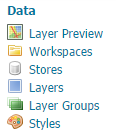
\includegraphics[width=0.25\textwidth]{Figures/Data.png}
	  \vspace{-10pt}
	\caption{\label{fig:data}Data section of navigator}
	  \vspace{-10pt}
\end{wrapfigure}
This section will give a step by step guide of how to create a visual geospacial representation using the pre-aggregated index of the example dataset. This will be done using GeoServer, specifically the GeoServer web administration interface. This section offers are concrete version of the deployment discussed in \Fref{sec:deployment}.

\Fref{fig:data} shows the \lstinline|Data| section of the navigator which can be found on the left hand side of the web administration interface. The links in this section will be used to navigate between different pages needed to configure the whole setup.

\subsubsection{Add Source}
A data source is added in the following manor:
\begin{enumerate}
	\item Click on the \lstinline|Stores| link in the \lstinline|Data| section shown in \Fref{fig:data}.
	\item The \lstinline|Stores| will open, the top of the page will look like \Fref{fig:newstore}, click on the \lstinline|Add new Store| link.
	\item A selection of different \lstinline|Vector Data Sources| is now available. Select \lstinline|NeoGeo Aggregate| as shown in \Fref{fig:storetype}. 
\end{enumerate}
\begin{figure}[h]
	\centering
	\subfigure[Add new store \label{fig:newstore}]{
		\raisebox{8mm}{
		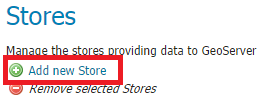
\includegraphics[scale=0.6]{Figures/AddNewStores.png} }}
	\subfigure[Select data source type \label{fig:storetype}]{
		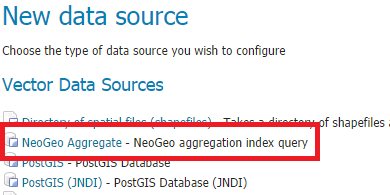
\includegraphics[scale=0.6]{Figures/StoreType.png} }
	\caption{Adding new \lstinline|Store| to GeoServer}
\end{figure}

\begin{enumerate}[resume]
	\item After selecting \lstinline|NeoGeo Aggregate| as \lstinline|Vector Data Source| a page like \Fref{fig:createstore} will open. Fill in all the fields as shown, some values may differ depending on how the database is setup. More exact information can be found in \Fref{sec:addingsource}.
	\item Once everything is filled out click the \lstinline|Save| button. This leads to page where \lstinline|Layers| can be published. However before that is done first the \lstinline|Style| should be imported.
\end{enumerate}

\begin{figure}[h!tb]
	\centering
		\begin{minipage}{0.5\textwidth}
			\centering 	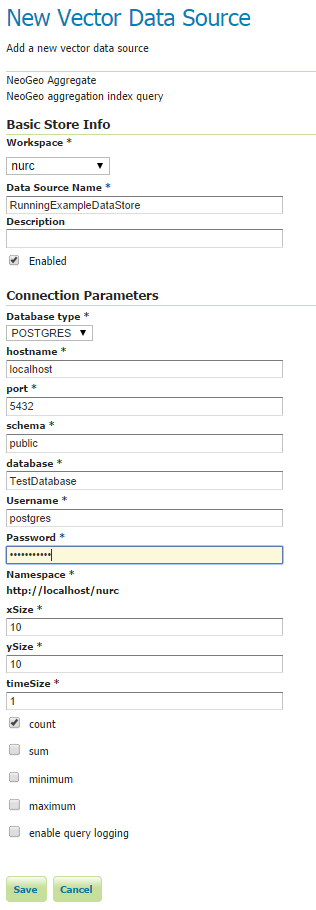
\includegraphics[width=.94\textwidth]{Figures/CreateStore.png}
			\caption{\label{fig:createstore}\lstinline|New Vector Data Source|}
		\end{minipage}\hfill
		\begin{minipage}{0.5\textwidth}
			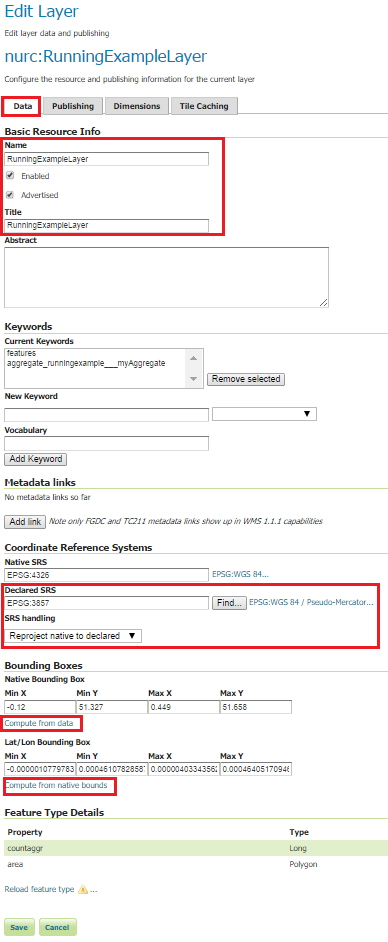
\includegraphics[width=1.11\textwidth]{Figures/EditLayer_Data.png}
			\caption{\label{fig:editlayerdata}\lstinline|Edit Layer| page}
		\end{minipage}
\end{figure}

\clearpage
\subsubsection{Import Style}
Importing a style is done as follows:
\begin{enumerate}[resume]
	\item Click on the \lstinline|Styles| link in the \lstinline|Data| section shown in \Fref{fig:data}.
	\item Click on the \lstinline|Add a new style| button which will go a page similar to \Fref{fig:styleimport} although empty.
	\item Import the \lstinline|RunningExampleSLD.xml| file by using the \lstinline|Choose File| button then the \lstinline|Upload...| link highlighted in red in \Fref{fig:styleimport}.
	\item Once the style has been upload the \lstinline|New style| page should look like \Fref{fig:styleimport}.
	\item Press the \lstinline|Save| button.
\end{enumerate}
The style used in this example has been imported in GeoServer and now the layer is ready to published.
\begin{figure}[h!]
	\centering
	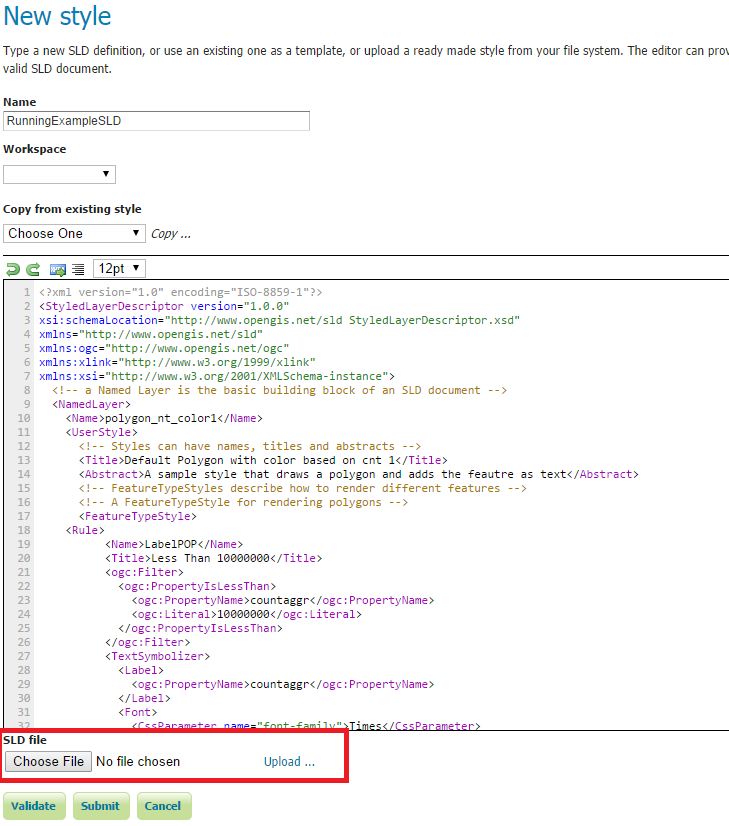
\includegraphics[scale=0.5]{Figures/NewStyleImport.png}
	\caption{\label{fig:styleimport}Importing SLD style from file}
\end{figure}

\pagebreak
\subsubsection{Create Layer}
\begin{figure}[h!]
	\centering
	\vspace{-15pt}
	\includegraphics[width=\textwidth]{Figures/Publishlayer.png}
	\vspace{-5pt}
	\caption{Publishing a \lstinline|Layer|\label{fig:publishlayer}}
\end{figure}
\noindent Creating a new layer is done as follows:
\vspace{10pt}

\begin{minipage}{.45\textwidth}
	\begin{enumerate}[resume]
		\item Click on the \lstinline|Layers| link in the \lstinline|Data| section shown in \Fref{fig:data}.
		\item This opens the \lstinline|Layers| page, here click on the \lstinline|Add a new resource| button. This open a page similar to \Fref{fig:publishlayer}.
		\item Select the \lstinline|Publish| action for the example layer.
		\item A page like \Fref{fig:editlayerdata} will open. Set highlighted fields to match \Fref{fig:editlayerdata}. More exact information about these fields can be found in \Fref{sec:addinglayers}.
		\item After the fields in the \lstinline|Data| are filled in, go to the \lstinline|Publishing| tab, see \Fref{fig:layerpublish}.
		\item Set the  default style to \lstinline|RunningExampleSLD| like in \Fref{fig:layerpublish}.
		\item Press the \lstinline|Save| button.
	\end{enumerate}
\end{minipage}\hfill
\begin{minipage}{.45\textwidth}
	\begin{figure}[H]
		\centering
		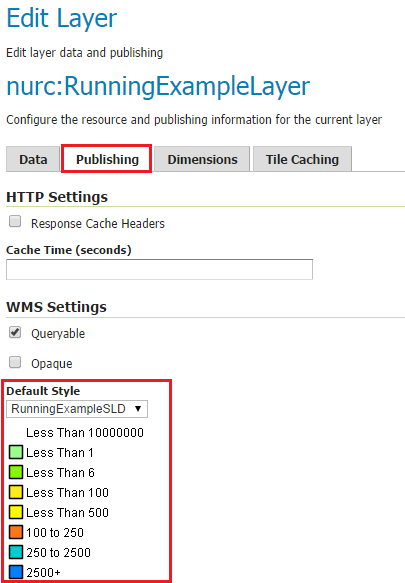
\includegraphics[width=\textwidth]{Figures/EditLayer_Publishing.png}
		\vspace{-5pt}
		\caption{Adding a \lstinline|Style| to the \lstinline|Layer| \label{fig:layerpublish}}
	\end{figure}
\end{minipage}

\vspace{10pt}
\noindent A layer for the example dataset has now been created and is ready to be viewed.


\pagebreak
\subsubsection{View Layer}
\begin{figure}[h!]
	\centering
	\vspace{-15pt}
	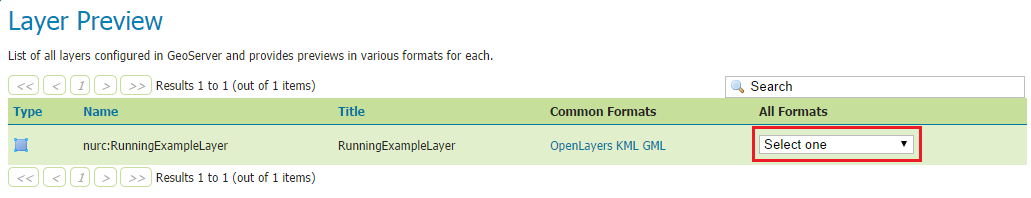
\includegraphics[width=\textwidth]{Figures/LayerPreview.png}
	\vspace{-25pt}
	\caption{Previewing a \lstinline|Layer|\label{fig:preview}}
\end{figure}
\noindent The final GeoServer step is to preview the layer. The preview only shows the highest granularity of the aggregation index. Getting a preview of a layer is done as follows:
\begin{enumerate}[resume]
	\item Click on the \lstinline|Layer Preview| link in the \lstinline|Data| section shown in \Fref{fig:data}.
	\item The \lstinline|Layer Preview| page opens which displays all viewable layers like in \Fref{fig:preview}.
	\item A preview format need to be selected from the drop-down menu highlighted in \Fref{fig:preview}.
	\item Select a \lstinline|WMS| preview format such as \lstinline|PNG|.
	\item A new web page will load (this might a few seconds depending on if the server side extension is enabled).
	\item The final result will look like \Fref{fig:result}.
\end{enumerate}
The layer which shows the example dataset is now complete. The values of each square in the layer is calculated using the pre-aggregate index of the dataset. See \ref{sec:clientsidedev} to learn how the layer can be used in combination with other tools such as OpenLayers\footnote{\url{http://openlayers.org/}} to create a dynamic map which updates data on the fly.
\begin{figure}[h!]
	\centering
	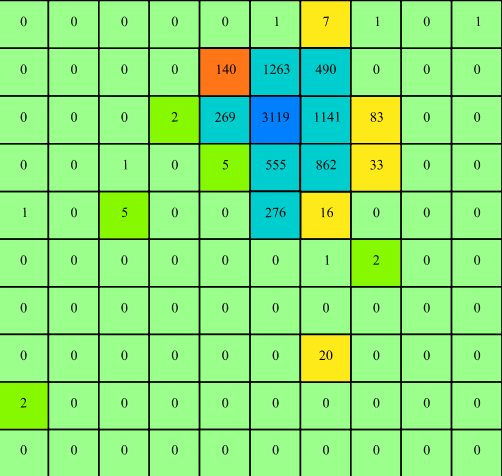
\includegraphics[width=0.45\textwidth]{Figures/FinalResult.png}
	\vspace{-5pt}
	\caption{Preview of whole dataset \label{fig:result}}
\end{figure}